\section{Resultados}\label{sec:resultados}

\subsection{\label{sub:data}Datos}\label{subsec:label{sub:data}datos}

En esta secci�n, las tablas~\ref{tab:1-t1-20},~\ref{tab:1-t1-45},~\ref{tab:2-t1-20} y~\ref{tab:2-t1-45} muestran
las mediciones del tiempo tomadas para las longitudes, �ngulos y masas especificadas.

Se contaron 20 oscilaciones para la masa 1 y 10 oscilaciones para la masa 2.

En cada tabla, se muestra la media de los 3 valores, o valor esperado de $t$, $\langle t \rangle$.
Tambi�n la dispersi�n de los datos  $D_m$, calculada como:
\begin{equation}
    D_m = \frac{x_{\text{m�x}} - x_{\text{m�n}}}{2}
\end{equation}

\begin{table}[tbh]
    \caption{Masa 1 - $20 \text{\textdegree}$ - Tiempo.}
    \label{tab:1-t1-20}
    \begin{centering}
        \begin{tabular}{|P{27px}|P{26px}P{26px}P{26px}|P{26px}P{26px}|}
            \hline
            $l$\,(mm)  & $t_1$\,(s) & $t_2$\,(s) & $t_3$\,(s) & $\langle t \rangle$\,(s) & $D_m$\,(s)                             \\
            \hline
            \csvreader[late after line= \\, /csv/separator=semicolon ]{./files/data/1-t1-20.csv}{}% use head of csv as column names
            {\csvcolii & \csvcoliii & \csvcoliv  & \csvcolv   & \csvcolvi                & \csvcolvii}% specify your columns here
            \hline
        \end{tabular}
    \end{centering}
\end{table}

\begin{table}[tbh]
    \caption{Masa 1 - $45 \text{\textdegree}$ - Tiempo.}
    \label{tab:1-t1-45}
    \begin{centering}
        \begin{tabular}{|P{27px}|P{26px}P{26px}P{26px}|P{26px}P{26px}|}
            \hline
            $l$\,(mm)  & $t_1$\,(s) & $t_2$\,(s) & $t_3$\,(s) & $\langle t \rangle$\,(s) & $D_m$\,(s)                             \\
            \hline
            \csvreader[late after line= \\, /csv/separator=semicolon ]{./files/data/1-t1-45.csv}{}% use head of csv as column names
            {\csvcolii & \csvcoliii & \csvcoliv  & \csvcolv   & \csvcolvi                & \csvcolvii}% specify your columns here
            \hline
        \end{tabular}
    \end{centering}
\end{table}

\begin{table}[tbh]
    \caption{Masa 2 - $20 \text{\textdegree}$ - Tiempo.}
    \label{tab:2-t1-20}
    \begin{centering}
        \begin{tabular}{|P{27px}|P{26px}P{26px}P{26px}|P{26px}P{26px}|}
            \hline
            $l$\,(mm)  & $t_1$\,(s) & $t_2$\,(s) & $t_3$\,(s) & $\langle t \rangle$\,(s) & $D_m$\,(s)                             \\
            \hline
            \csvreader[late after line= \\, /csv/separator=semicolon ]{./files/data/2-t1-20.csv}{}% use head of csv as column names
            {\csvcolii & \csvcoliii & \csvcoliv  & \csvcolv   & \csvcolvi                & \csvcolvii}% specify your columns here
            \hline
        \end{tabular}
    \end{centering}
\end{table}

\begin{table}[tbh]
    \caption{Masa 2 - $45 \text{\textdegree}$ - Tiempo.}
    \label{tab:2-t1-45}
    \begin{centering}
        \begin{tabular}{|P{27px}|P{26px}P{26px}P{26px}|P{26px}P{26px}|}
            \hline
            $l$\,(mm)  & $t_1$\,(s) & $t_2$\,(s) & $t_3$\,(s) & $\langle t \rangle$\,(s) & $D_m$\,(s)                             \\
            \hline
            \csvreader[late after line= \\, /csv/separator=semicolon ]{./files/data/2-t1-45.csv}{}% use head of csv as column names
            {\csvcolii & \csvcoliii & \csvcoliv  & \csvcolv   & \csvcolvi                & \csvcolvii}% specify your columns here
            \hline
        \end{tabular}
    \end{centering}
\end{table}

%\FloatBarrier

\subsection{\label{sub:results}An�lisis}\label{subsec:label{sub:results}analisis}

Fij�ndonos en los valores obtenidos de la dispersi�n $D_m$, un valor razonable del error absoluto en la medici�n de los tiempos es $\pm 0.2\,s$.

Las tablas~\ref{tab:1-t3-20},~\ref{tab:1-t3-45},~\ref{tab:2-t3-20} y~\ref{tab:2-t3-45} muestran el periodo calculado a partir de los datos anteriores.

\begin{table}[tbh]
    \caption{Masa 1 - 20\textdegree\;- Periodo.}
    \label{tab:1-t3-20}
    \begin{centering}
        \begin{tabular}{|P{56px}|P{67px}|P{67px}|}
            \hline
            $l$\,(mm) & $t$\,(s)  & $T = t / n$\,(s)                       \\
            \hline
            \csvreader[late after line= \\, /csv/separator=semicolon ]{./files/data/1-t3-20.csv}{}% use head of csv as column names
            {\csvcoli & \csvcolii & \csvcoliii}% specify your columns here
            \hline
        \end{tabular}
    \end{centering}
\end{table}

\begin{table}[tbh]
    \caption{Masa 1 - 45\textdegree\;- Periodo.}
    \label{tab:1-t3-45}
    \begin{centering}
        \begin{tabular}{|P{56px}|P{67px}|P{67px}|}
            \hline
            $l$\,(mm) & $t$\,(s)  & $T = t / n$\,(s)                       \\
            \hline
            \csvreader[late after line= \\, /csv/separator=semicolon ]{./files/data/1-t3-45.csv}{}% use head of csv as column names
            {\csvcoli & \csvcolii & \csvcoliii}% specify your columns here
            \hline
        \end{tabular}
    \end{centering}
\end{table}

\begin{table}[tbh]
    \caption{Masa 2 - 20\textdegree\;- Periodo.}
    \label{tab:2-t3-20}
    \begin{centering}
        \begin{tabular}{|P{56px}|P{67px}|P{67px}|}
            \hline
            $l$\,(mm) & $t$\,(s)  & $T = t / n$\,(s)                       \\
            \hline
            \csvreader[late after line= \\, /csv/separator=semicolon ]{./files/data/2-t3-20.csv}{}% use head of csv as column names
            {\csvcoli & \csvcolii & \csvcoliii}% specify your columns here
            \hline
        \end{tabular}
    \end{centering}
\end{table}

\begin{table}[tbh]
    \caption{Masa 2 - 45\textdegree\;- Periodo.}
    \label{tab:2-t3-45}
    \begin{centering}
        \begin{tabular}{|P{56px}|P{67px}|P{67px}|}
            \hline
            $l$\,(mm) & $t$\,(s)  & $T = t / n$\,(s)                       \\
            \hline
            \csvreader[late after line= \\, /csv/separator=semicolon ]{./files/data/2-t3-45.csv}{}% use head of csv as column names
            {\csvcoli & \csvcolii & \csvcoliii}% specify your columns here
            \hline
        \end{tabular}
    \end{centering}
\end{table}


Las figuras~\ref{fig:1-20-1},~\ref{fig:1-45-1},~\ref{fig:2-20-1} y~\ref{fig:2-45-1} muestran las gr�ficas del periodo
frente a la ra�z cuadrada de la longitud.

\begin{figure}[tbh]
    \begin{center}
        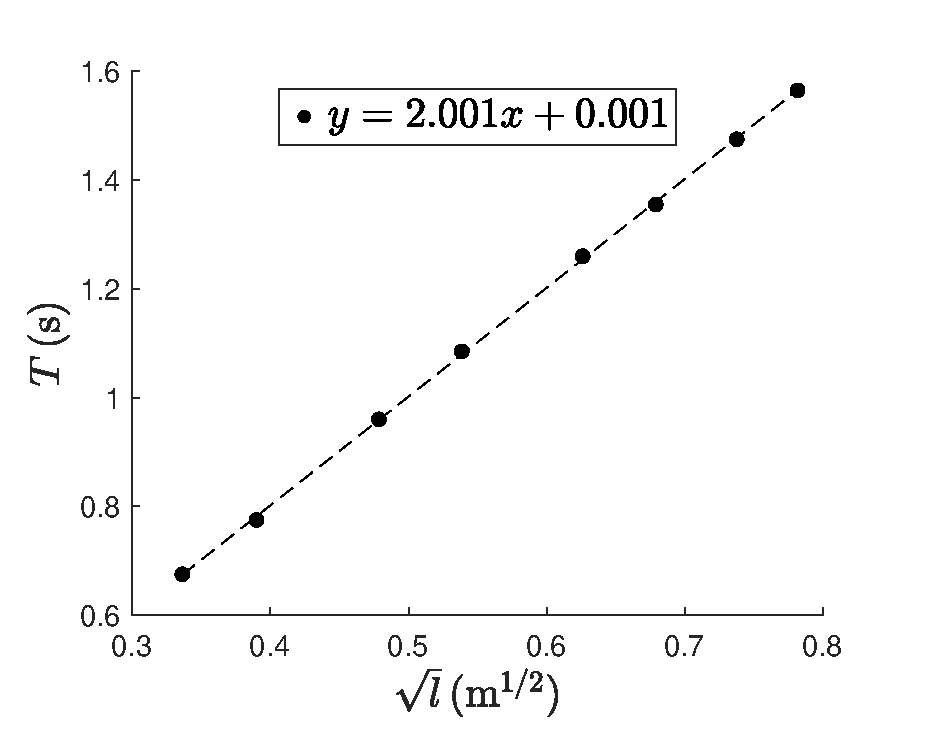
\includegraphics[width=0.8\columnwidth]{files/images/1-20-1}
    \end{center}
    \caption{Masa 1 - 20\textdegree\;- $T$ frente a $\sqrt {l}$.}
    \label{fig:1-20-1}
\end{figure}

\begin{figure}[tbh]
    \begin{center}
        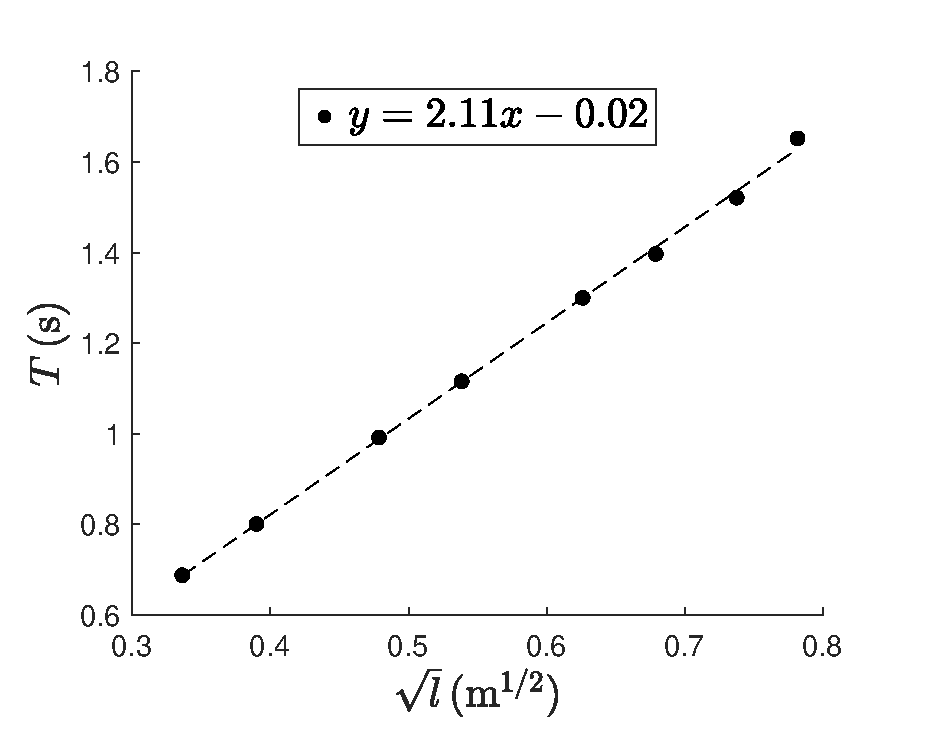
\includegraphics[width=0.8\columnwidth]{files/images/1-45-1}
    \end{center}
    \caption{Masa 1 - 45\textdegree\;- $T$ frente a $\sqrt {l}$.}
    \label{fig:1-45-1}
\end{figure}

\begin{figure}[tbh]
    \begin{center}
        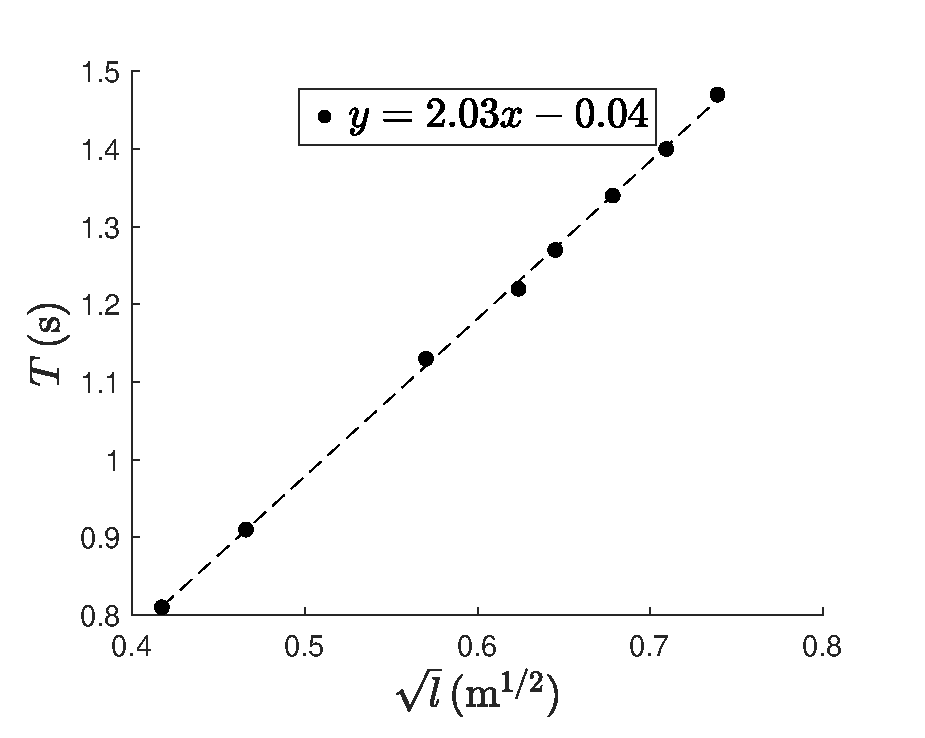
\includegraphics[width=0.8\columnwidth]{files/images/2-20-1}
    \end{center}
    \caption{Masa 2 - 20\textdegree\;- $T$ frente a $\sqrt {l}$.}
    \label{fig:2-20-1}
\end{figure}

\begin{figure}[tbh]
    \begin{center}
        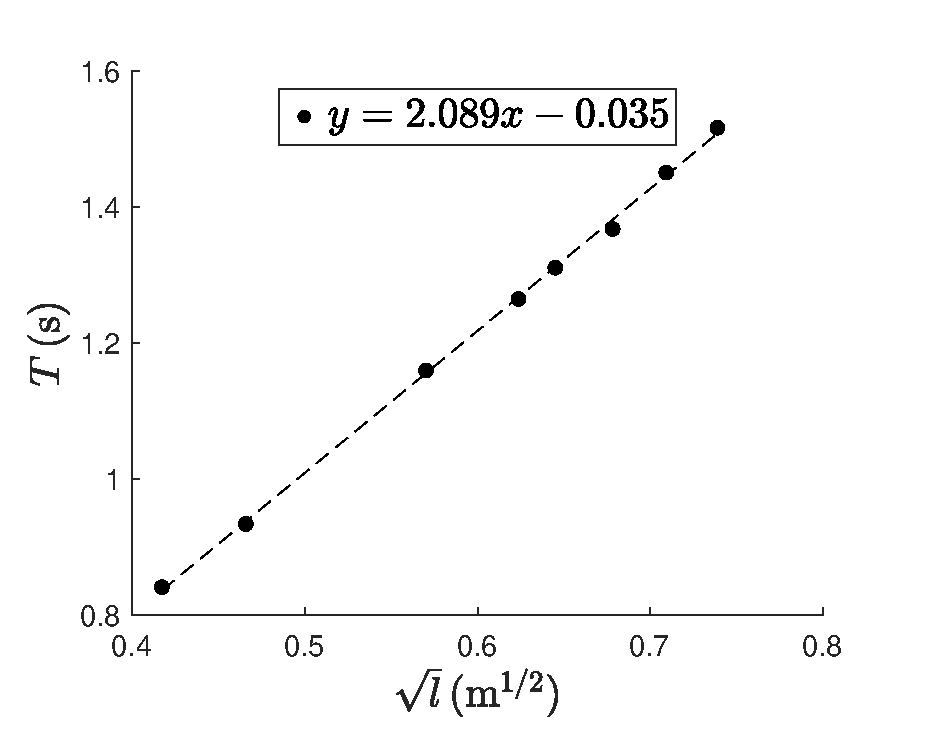
\includegraphics[width=0.8\columnwidth]{files/images/2-45-1}
    \end{center}
    \caption{Masa 2 - 45\textdegree\;- $T$ frente a $\sqrt {l}$.}
    \label{fig:2-45-1}
\end{figure}

La pendiente de las gr�ficas~\ref{fig:1-20-1},~\ref{fig:1-45-1},~\ref{fig:2-20-1} y~\ref{fig:2-45-1}
incluida su desviaci�n est�ndar como error, es:

\begin{table}[tbh]
    \caption{$g$}
    \label{tab:g}
    \begin{centering}
        \begin{tabular}{|P{56px}|P{67px}|P{67px}|}
            \hline
            & $a\;\text{(s/m$^{1/2}$)}$ & $g\;\text{(m/s$^2$)}$ \\
            \hline
            Masa 1, 20\textdegree & 2,000 \pm\; 0,011         & 9,87 \pm\; 0,11       \\
            Masa 1, 45\textdegree & 2,11 \pm\; 0,03           & 8,87 \pm\; 0,25       \\
            Masa 2, 20\textdegree & 2,034 \pm\; 0,017         & 9,54 \pm\; 0,16       \\
            Masa 2, 45\textdegree & 2,09 \pm\; 0,03           & 9,04 \pm\; 0,26       \\
            \hline
        \end{tabular}
    \end{centering}
\end{table}




Las figuras~\ref{fig:1-20-2},~\ref{fig:1-45-2},~\ref{fig:2-20-2} y~\ref{fig:2-45-2} muestran las gr�ficas del periodo
al cuadrado frente a la longitud.

\begin{figure}[tbh]
    \begin{center}
        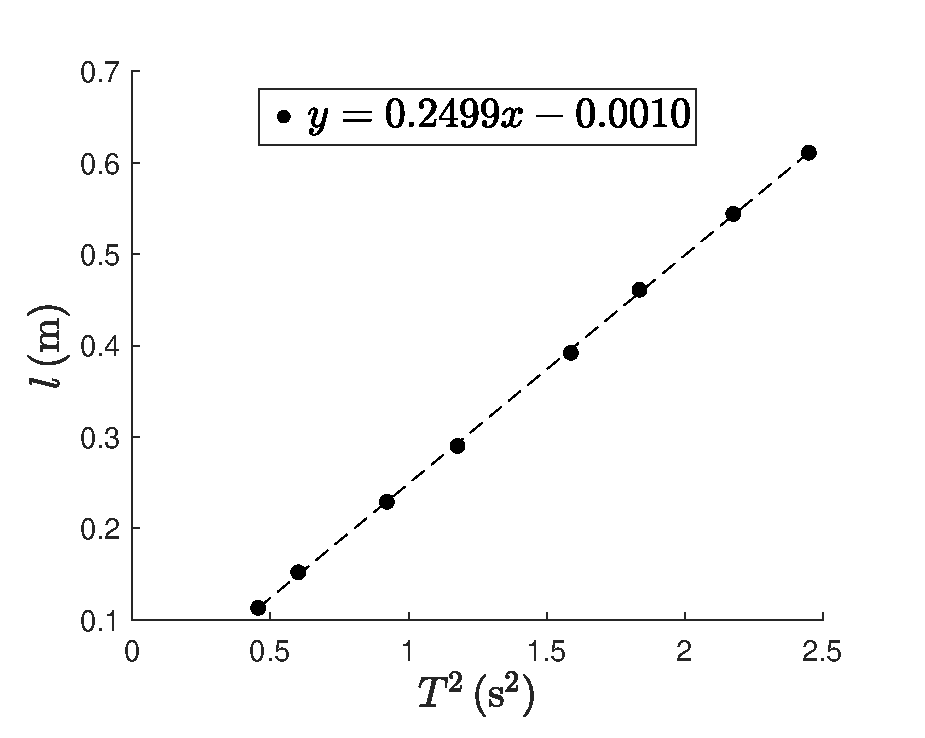
\includegraphics[width=0.8\columnwidth]{files/images/1-20-2}
    \end{center}
    \caption{Masa 1 - 20\textdegree\;- $l$ frente a $T^2$.}
    \label{fig:1-20-2}
\end{figure}

\begin{figure}[tbh]
    \begin{center}
        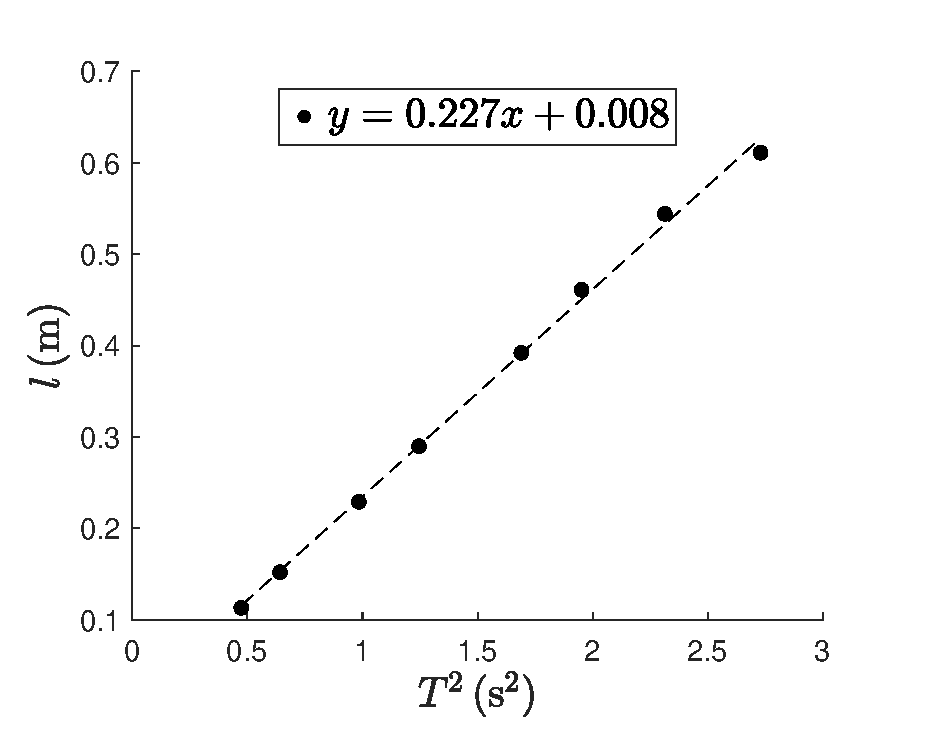
\includegraphics[width=0.8\columnwidth]{files/images/1-45-2}
    \end{center}
    \caption{Masa 1 - 45\textdegree\;- $l$ frente a $T^2$.}
    \label{fig:1-45-2}
\end{figure}

\begin{figure}[tbh]
    \begin{center}
        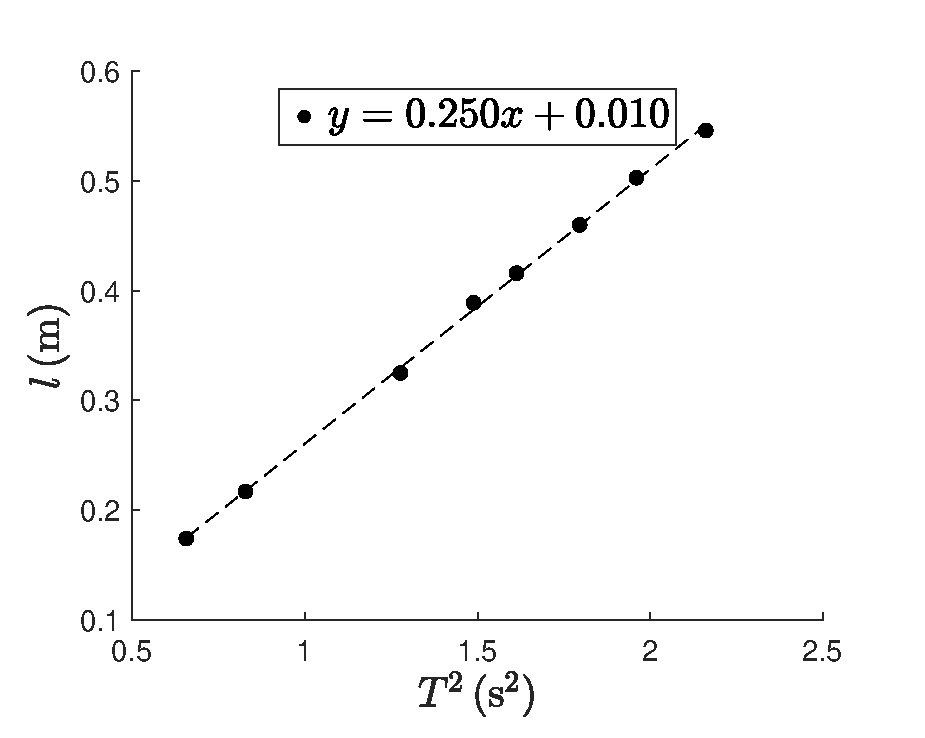
\includegraphics[width=0.8\columnwidth]{files/images/2-20-2}
    \end{center}
    \caption{Masa 2 - 20\textdegree\;- $l$ frente a $T^2$.}
    \label{fig:2-20-2}
\end{figure}

\begin{figure}[tbh]
    \begin{center}
        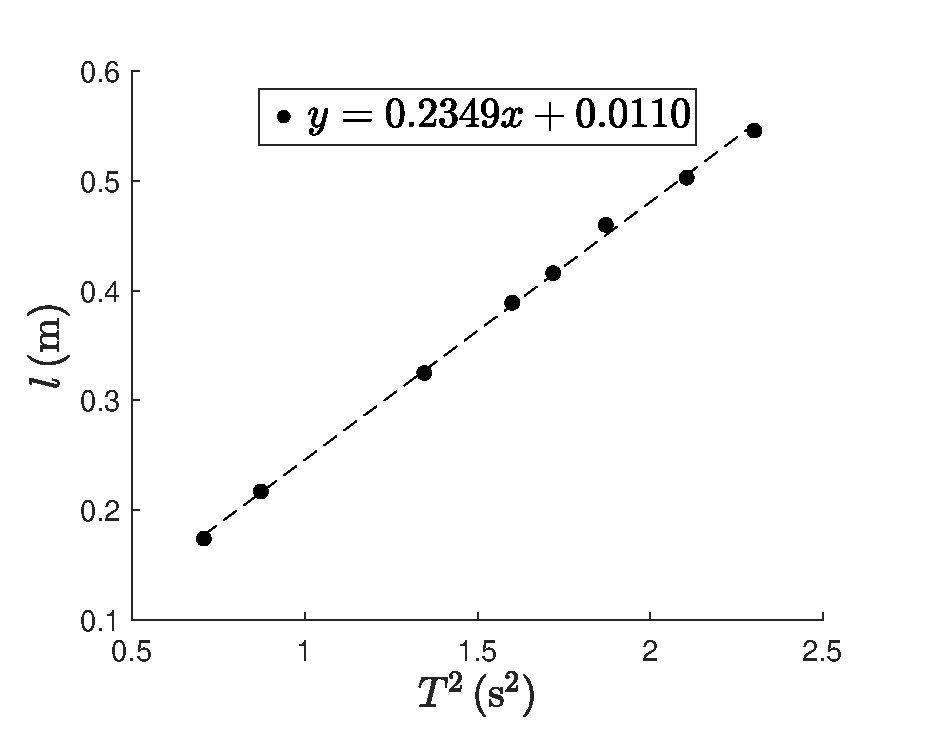
\includegraphics[width=0.8\columnwidth]{files/images/2-45-2}
    \end{center}
    \caption{Masa 2 - 45\textdegree\;- $l$ frente a $T^2$.}
    \label{fig:2-45-2}
\end{figure}

La pendiente de las gr�ficas~\ref{fig:1-20-2},~\ref{fig:1-45-2},~\ref{fig:2-20-2} y~\ref{fig:2-45-2}
incluida su desviaci�n est�ndar como error, es:

\begin{table}[tbh]
    \caption{$g$}
    \label{tab:g2}
    \begin{centering}
        \begin{tabular}{|P{56px}|P{67px}|P{67px}|}
            \hline
            & $a\;\text{(s/m$^{1/2}$)}$ & $g\;\text{(m/s$^2$)}$ \\
            \hline
            Masa 1, 20\textdegree & 2,000 \pm\; 0,011         & 9,87 \pm\; 0,11       \\
            Masa 1, 45\textdegree & 2,11 \pm\; 0,03           & 8,87 \pm\; 0,25       \\
            Masa 2, 20\textdegree & 2,034 \pm\; 0,017         & 9,54 \pm\; 0,16       \\
            Masa 2, 45\textdegree & 2,09 \pm\; 0,03           & 9,04 \pm\; 0,26       \\
            \hline
        \end{tabular}
    \end{centering}
\end{table}



\begin{figure}[tbh]
    \begin{center}
        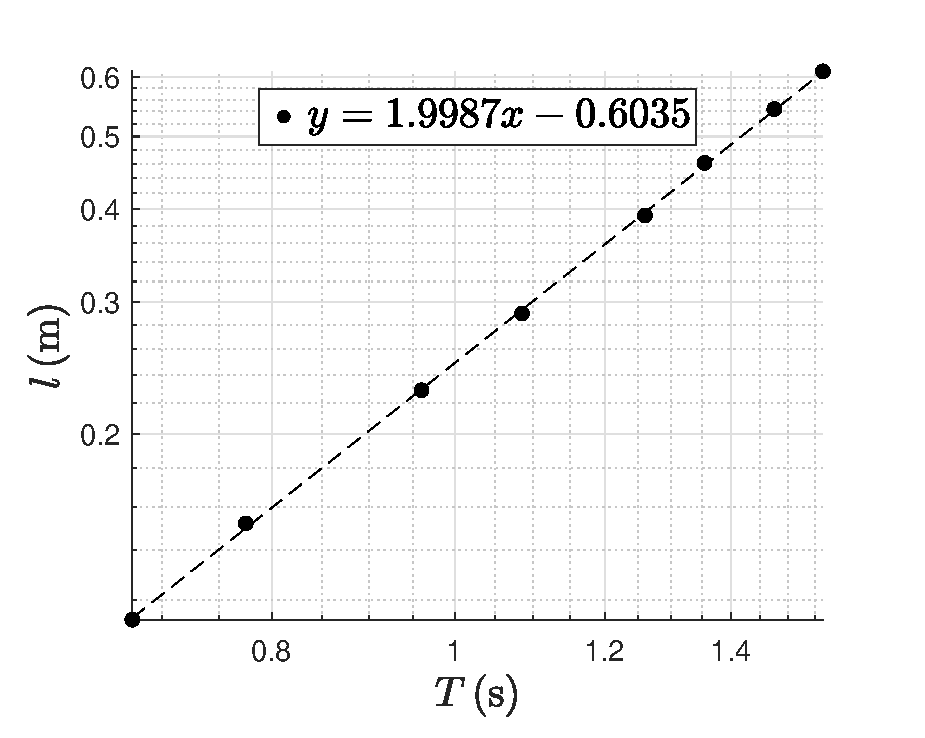
\includegraphics[width=0.8\columnwidth]{files/images/1-20-3}
    \end{center}
    \caption{Masa 1 - 20\textdegree\;- $l$ frente a $T$.}
    \label{fig:1-20-3}
\end{figure}

\begin{figure}[tbh]
    \begin{center}
        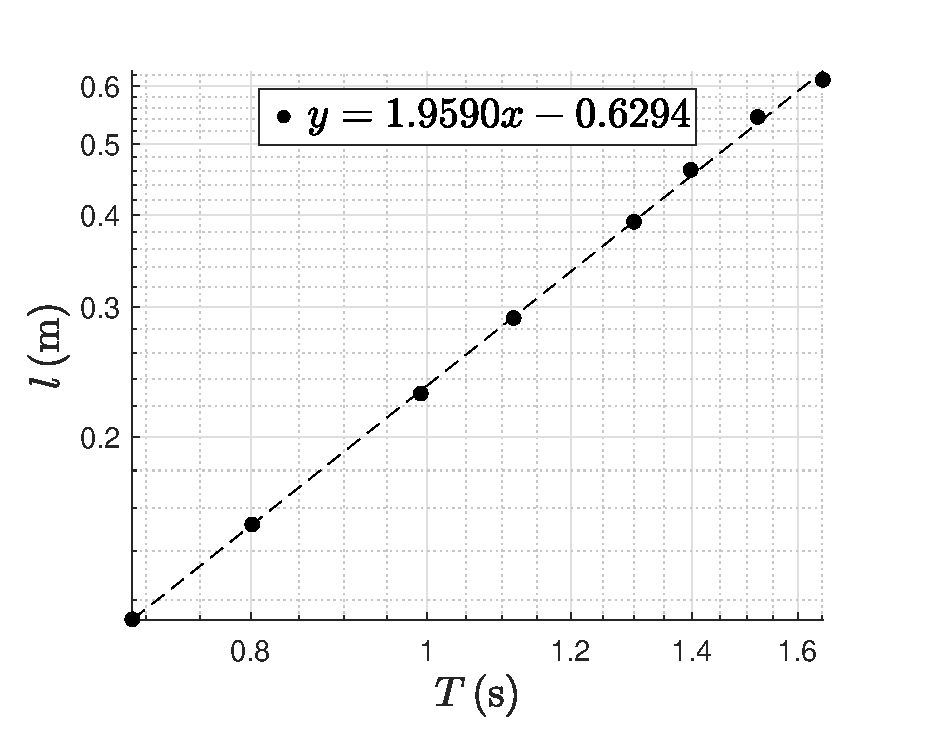
\includegraphics[width=0.8\columnwidth]{files/images/1-45-3}
    \end{center}
    \caption{Masa 1 - 45\textdegree\;- $l$ frente a $T$.}
    \label{fig:1-45-3}
\end{figure}

\begin{figure}[tbh]
    \begin{center}
        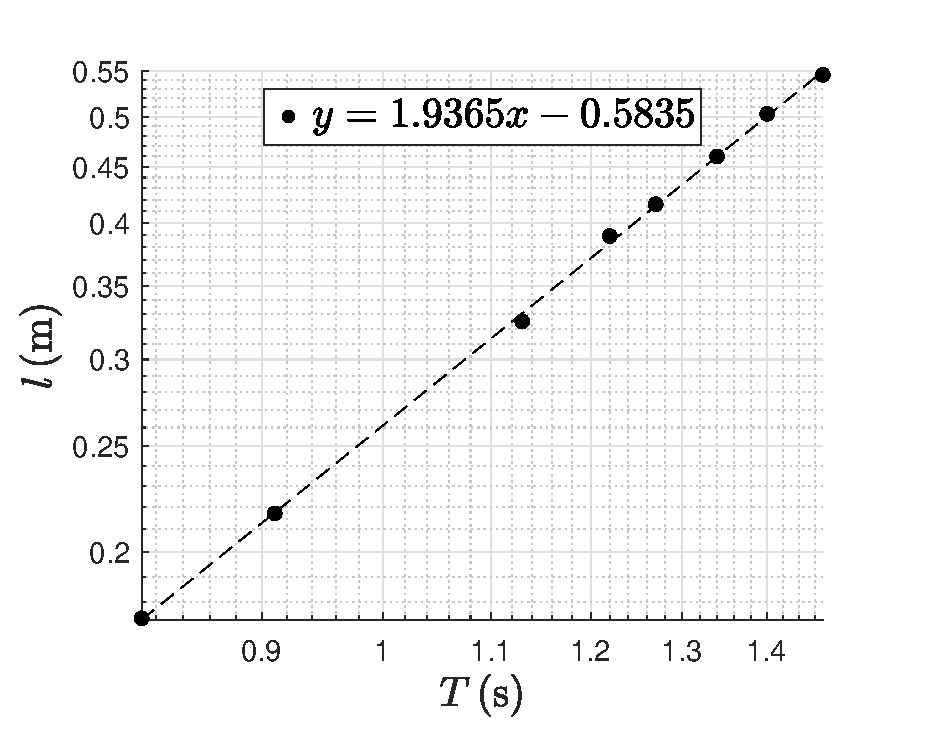
\includegraphics[width=0.8\columnwidth]{files/images/2-20-3}
    \end{center}
    \caption{Masa 2 - 20\textdegree\;- $l$ frente a $T$.}
    \label{fig:2-20-3}
\end{figure}

\begin{figure}[tbh]
    \begin{center}
        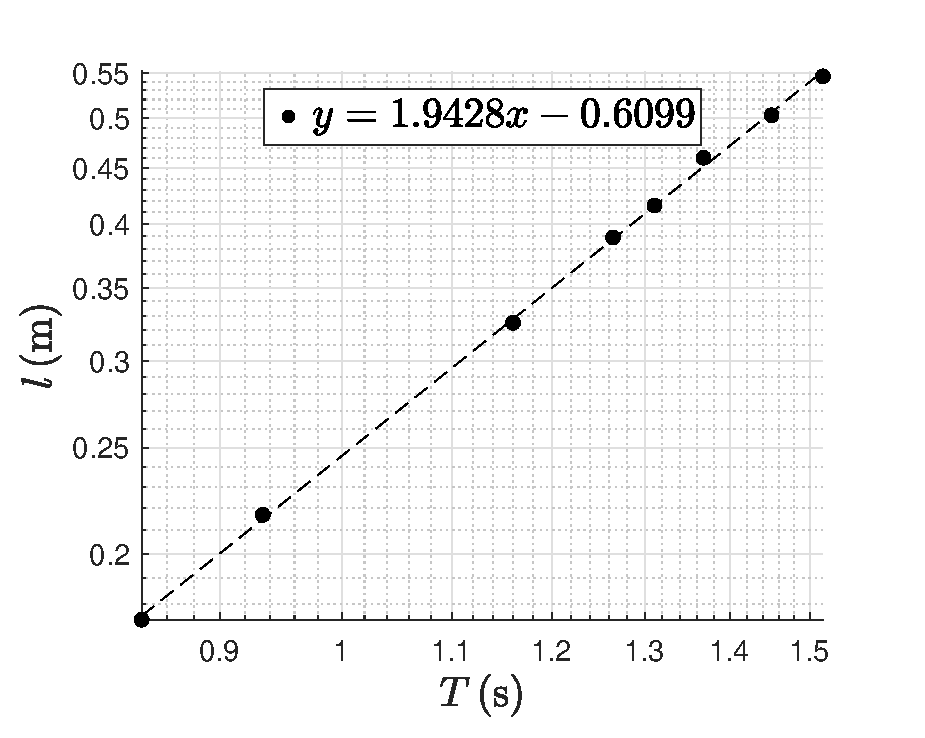
\includegraphics[width=0.8\columnwidth]{files/images/2-45-3}
    \end{center}
    \caption{Masa 2 - 45\textdegree\;- $l$ frente a $T$.}
    \label{fig:2-45-3}
\end{figure}

Se agrupan en una l�nea de pendiente 2.

Observamos que los tiempos para amplitudes grandes son mayores que para amplitudes peque�as.

Tambi�n observamos que los tiempos medidos para las dos masas coinciden.


